\documentclass[12pt,letterpaper,fleqn]{article}

%       amslatex provides nice math extensions for typesetting mathematics
\usepackage{amsmath}
\usepackage{amsfonts}
\usepackage{tmmaths}
\usepackage{sympytex}

%       pstricks provides powerful environments for incorporating postscript into a
%       TeX/LaTeX document. You must have a postscript printer and a package like
%       dvips to convert the DVI file to a PS file.
%\usepackage{pst-all}
%\usepackage{pstricks,pst-plot}
%\usepackage{pst-coil,pst-node}

%  This package provides native tex support for numbered grids. The syntax is:
%  \graphpaper[spc](x_lowleft,y_lowleft)(x_upperright,y_upperright)

%\usepackage{graphpap}
%\usepackage{float}

%  The package below must be initialized with "\initfloatingfigs" immediately after the
%  "\begin{document} command.
%\usepackage{floatfig}

\usepackage{graphicx}
\graphicspath{{i:/mytex/graphics}}
\DeclareGraphicsExtensions{.ps,.eps}

%       tst is a package for the creation of exams, quizzes and tests. the include
%       file mathstuf (see below) provides many abbreviations for these environments.
%\usepackage{tst}

%       epsfig is a package which provides for the inclusion of Encapsulated PostScript
%       files in a document.
%\usepackage{epsfig}
%\usepackage{epic,eepic}
\include{mathstuf}
\usepackage[total={7.25in,10in},top=0.25in,left=0.75in,includehead]{geometry}
\usepackage{fancyhdr}
\pagestyle{fancy}
\lhead{Math 252}
\rhead{\large Name\makebox[2in]{\hrulefill}}
\chead{\LARGE Exploration 3}
%\lfoot{\today}
\cfoot{}
%\rfoot{\thepage}
\renewcommand{\headrulewidth}{0.4pt}
\renewcommand{\footrulewidth}{0.4pt}
\setlength{\parindent}{0pt}
\setlength{\parskip}{2ex}

\newcounter{tf}[enumi]
\newenvironment{tf}[0]{\begin{list}%
{\alph{tf}. \makebox[5em]{True\hfill False}}%
{\usecounter{tf}\setlength{\labelwidth}{7em}%
\setlength{\leftmargin}{3.5cm}%
\setlength{\labelsep}{1cm}}}%
{\end{list}}

%\usepackage{epic,eepic}
\newcommand{\numline}{%
%\newcounter{mark}%
%\setcounter{mark}{-1}%
\setlength{\unitlength}{0.1in}%
\begin{picture}(0,0)%
\thicklines%
\put(0,0){\line(1,0){60}}%
\multiput(0,0)(10,0){7}{\line(0,-1){1}%
\makebox(0,-1.5)[t]{\arabic{mark}}\stepcounter{mark}}%
%
\thinlines%
\multiput(0,0)(5,0){12}{\line(0,-1){0.5}}%
\multiput(0,0)(1,0){60}{\line(0,-1){0.3}}%
%\put(-5,265){\makebox(0,0)[l]{{\bf cm}}}%
\end{picture}}%

\newcommand{\ds}{\displaystyle}
\usepackage{amsfonts}


\let\oldhat\hat
\renewcommand{\hat}[1]{\oldhat{\boldsymbol{\mathbf{#1}}}}
\newcommand{\lv}[1]{\ensuremath{\langle #1 \rangle}}
\renewcommand{\i}{\ensuremath{\hat{\imath}}}
\renewcommand{\j}{\ensuremath{\hat{\jmath}}}
\renewcommand{\k}{\ensuremath{\mathbf{\oldhat{k}}}}
\newcommand{\ora}[1]{\ensuremath{\overrightarrow{#1}}}
\renewcommand{\vec}[1]{\ensuremath{\mathbf{#1}}}
\renewcommand{\v}[1]{\ensuremath{\vec{#1}}}
\newcommand{\abs}[1]{\ensuremath{\lvert #1 \rvert}}

\usepackage{tabularx}
\usepackage{paralist}
\newcommand{\red}[1]{\textcolor{red}{#1}}
\newcommand{\blue}[1]{\textcolor{blue}{#1}}
% \newcommand{\ans}[1]{\quad\fbox{answer: \red{#1}}}
\newcommand{\ans}[1]{\mbox{{\bf Ans:} \blue{#1}}}
\newcommand{\dd}[2][]{\ensuremath{\frac{\text{d}#1}{\text{d}#2}}}
\newcommand{\eval}[2]{\ensuremath{\left.#1\right|_{#2}}}

\usepackage{wrapfig}

\begin{document}
Below is the graph of the speed $v$ of a bicycle (in mph) over a 20 minute time period; This is the same graph as in exploration 1. The purpose of this exploration is to find and plot the function $s(t)$ which gives the distance $s$ (in miles) travelled over the time interval $[0, t]$ minutes.
\begin{enumerate}
 \item Find an expression for the distance $s$ (in miles) travelled over a time interval $\Delta t$ minutes if the speed $v$ is \emph{constant} over that time interval.
 \item The speed $v$ is a constant 10 mph over the time interval $[0, 4]$ minutes. Find an expression for $s(t)$ for a time $t$ within this interval ($0 \leq t \leq 4$). Graph this part of the function $s$ over the interval $[0, 4]$. What does the slope of this part of the graph represent in the problem?
 \item Similarly, the speed has constant values of 20 mph, 16 mph and 6 mph over the time intervals (in minutes) $[4, 6]$, $[6, 12]$ and $[12, 20]$, respectively. Continue to plot the function $s$ over these successive intervals.
\end{enumerate}
\begin{figure}[h!]\hspace{0.25in}
 % \centering
 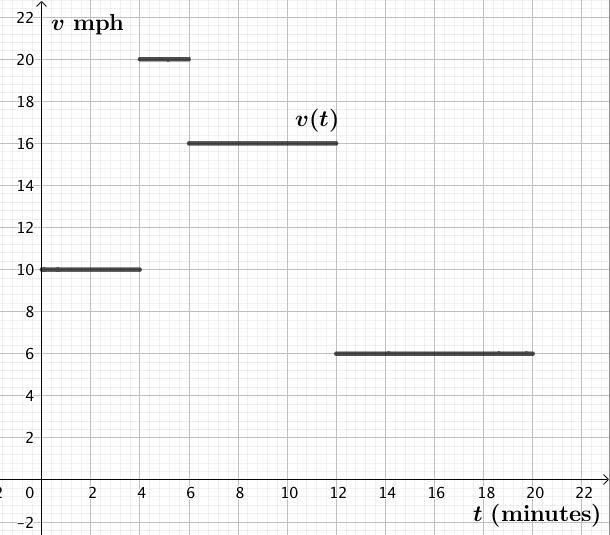
\includegraphics[width=0.3\textwidth]{img/speed_graph.png}
 % \caption{}
 % \label{}
\end{figure}
\begin{figure}[!htb]\hspace{0.25in}
	% \centering
	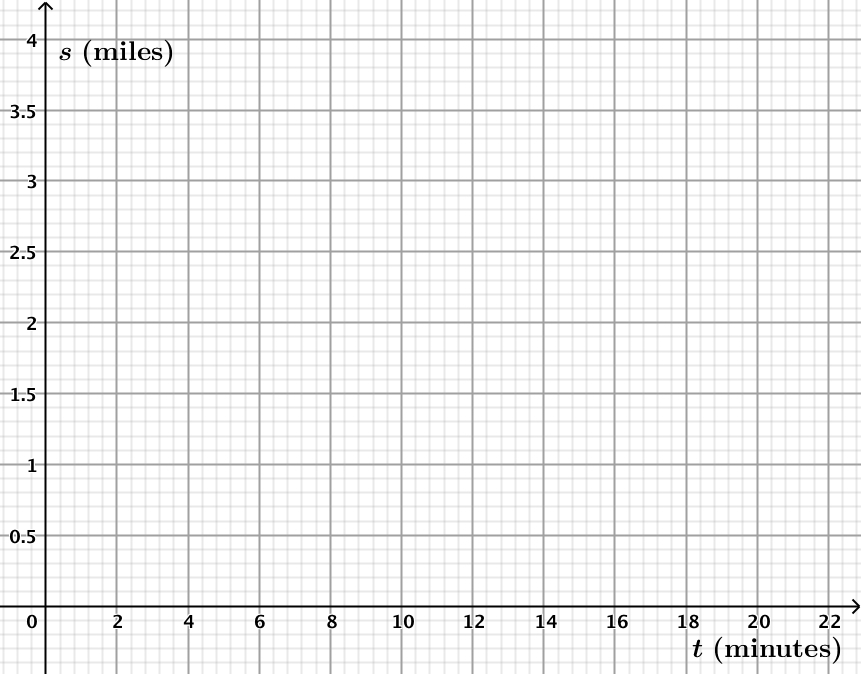
\includegraphics[width=0.7\textwidth]{img/distance.png}
	% \caption{}
	% \label{}
\end{figure}

\end{document}
